\documentclass{beamer}
\usetheme{Singapore}
\usepackage[utf8]{inputenc}
\usecolortheme{crane}
\usepackage{graphicx}
\usepackage{standalone}
\usepackage{tikz}
\usetikzlibrary{arrows}
\usetikzlibrary{decorations.markings}
\usetikzlibrary{calc}
\usetikzlibrary{shapes,snakes}
\usepackage{amsmath}
\usepackage{amsfonts}
\usepackage{amsthm}
\usepackage{mathtools}
\usepackage{tcolorbox}
\usepackage{float}
\usepackage{bm}
\usepackage{minted}
\usepackage{booktabs}

\definecolor{lightblue}{RGB}{124,190,255}
\definecolor{darkgreen}{RGB}{24,145,0}
\definecolor{darkorange}{RGB}{220,110,0}
\definecolor{bg}{RGB}{249, 251, 223}


\beamertemplatenavigationsymbolsempty
\setbeamerfont{caption}{size=\tiny}


\title
{Python for Operational Research in Healthcare}
\subtitle{\textit{There's a library for that...}}
\author{\textcolor{darkorange}{@GeraintPalmer}}
\date{PyCon UK 2017}
\titlegraphic{
\includegraphics[width=2.35cm]{cflogo}}

\begin{document}

\frame{\titlepage}

\begin{frame}
  \begin{center}
    
\includegraphics[width=0.22\textwidth]{barchart}\hspace{3mm}
    
\includegraphics[width=0.22\textwidth]{linechart}\hspace{3mm}
    
\includegraphics[width=0.22\textwidth]{division}\\
    \vspace{7mm}
    
\includegraphics[width=0.22\textwidth]{triangruler}\hspace{3mm}
    
\includegraphics[width=0.22\textwidth]{computer}\hspace{3mm}
    
\includegraphics[width=0.22\textwidth]{airplane}\\
  \end{center}
\end{frame}

\frame{
  \begin{center}
    
\includegraphics[width=0.5\textwidth]{importessay}
    \textcolor{darkorange}{\url{http://i.imgur.com/ZyeCO.jpg}}
  \end{center}
}

\begin{frame}[fragile]
  \frametitle{The Basics}
  \begin{center}
    \begin{tabular}{llrr}
    \toprule
    & Sex & Height & Weight \\
    \midrule
    0 & M & 187.306088 & 72.233276 \\
    1 & M & 170.595112 & 92.195728 \\
    2 & F & 157.637346 & 64.835601 \\
    3 & M & 162.010640 & 130.462244 \\
    4 & F & 154.017198 & 81.568846 \\
    $\vdots$ & $\vdots$ & $\vdots$ & $\vdots$ \\
    \bottomrule
  \end{tabular}
  \pause
  \small{
    \begin{minted}{python}
      >>> import scipy.stats

      >>> scipy.stats.ttest_ind(
      ...    df[df['Sex']=='M']['Height'],
      ...    df[df['Sex']=='F']['Height']
      ... ).pvalue
      0.070033630470421021
    \end{minted}
  }
  \end{center}
\end{frame}

\begin{frame}[fragile]
\frametitle{Machine Learning}
\begin{center}
  \only<1>{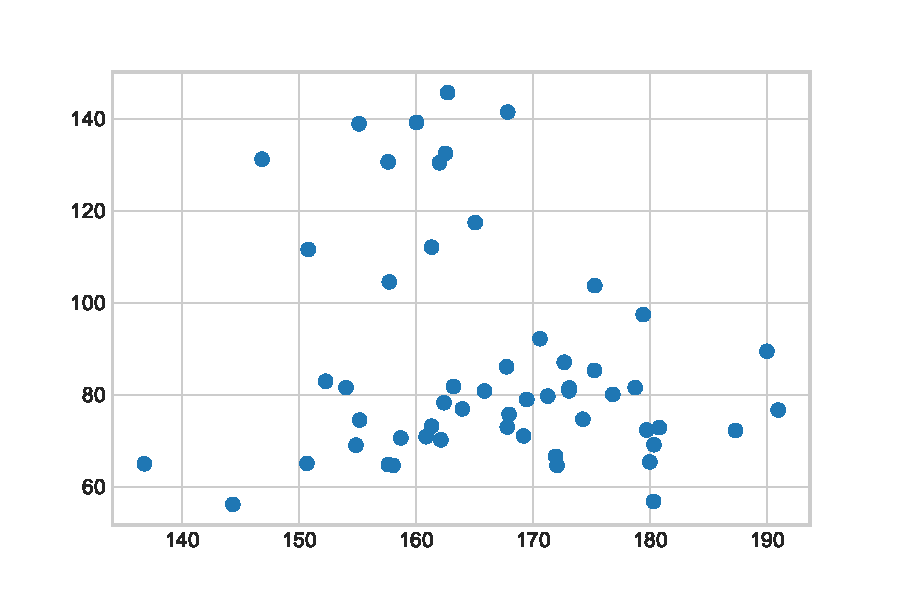
\includegraphics[width=0.6\textwidth]{heightweight}}
  \only<2>{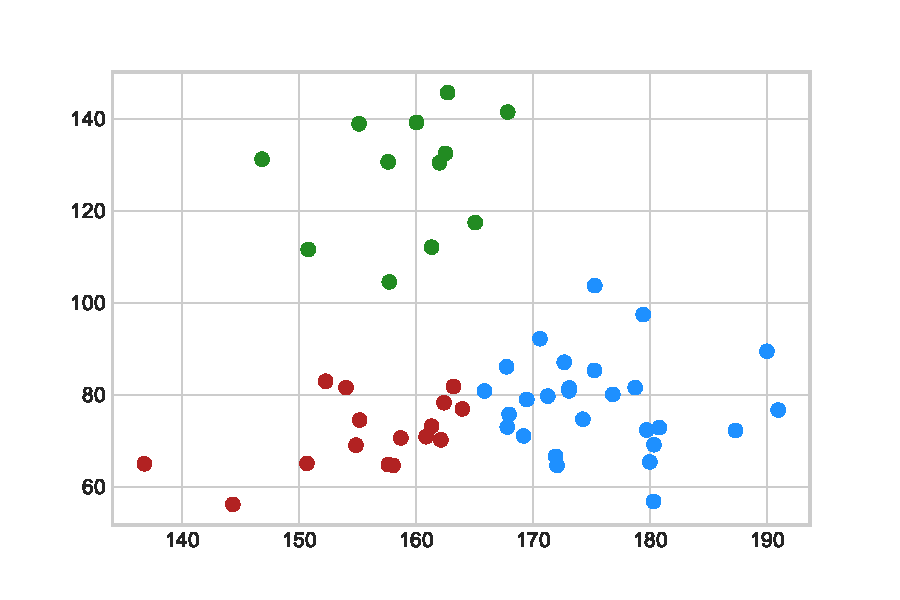
\includegraphics[width=0.6\textwidth]{heightweight_cluster}}
  \begin{minted}{python}
  >>> from sklearn.cluster import KMeans

  >>> kmeans = KMeans(n_clusters=3, random_state=0)
  >>> kmeans.fit(df[['Height', 'Weight']])
  >>> df['Cluster'] = kmeans.labels_
  \end{minted}
\end{center}
\end{frame}

\frame{
  \frametitle{Optimisation}
  \begin{center}
      \includestandalone[width=0.09\textwidth]{clock9}
      \includestandalone[width=0.09\textwidth]{clock10}
      \includestandalone[width=0.09\textwidth]{clock11}
      \includestandalone[width=0.09\textwidth]{clock12}
      \includestandalone[width=0.09\textwidth]{clock1}
      \includestandalone[width=0.09\textwidth]{clock2}
      \includestandalone[width=0.09\textwidth]{clock3}
      \includestandalone[width=0.09\textwidth]{clock4}
      \includestandalone[width=0.09\textwidth]{clock5}
      \includestandalone[width=0.09\textwidth]{clock6}\\
      \vspace{10mm}
      \includestandalone[width=0.4\textwidth]{fulltime}
      \hspace{10mm}
      \includestandalone[width=0.4\textwidth]{parttime}
  \end{center}
}

\begin{frame}
  $$\underline{x} = \left[F_9, F_{10}, F_{11}, P_9, P_{10}, P_{11}, P_{12}, P_{1}, P_{2}, P_{3}\right]$$

  $$C = \left[\text{\textsterling} 60, \text{\textsterling} 60, \text{\textsterling} 60, \text{\textsterling} 32, \text{\textsterling} 32, \text{\textsterling} 32, \text{\textsterling} 32, \text{\textsterling} 32, \text{\textsterling} 32, \text{\textsterling} 32\right]$$

  \begin{columns}
    \begin{column}{0.5\textwidth}
      $$A =
      \begin{bmatrix}{1}
        1 & 0 & 0 & 1 & 0 & 0 & 0 & 0 & 0 & 0 \\
        1 & 1 & 0 & 1 & 1 & 0 & 0 & 0 & 0 & 0 \\
        1 & 1 & 1 & 1 & 1 & 1 & 0 & 0 & 0 & 0 \\
        1 & 1 & 1 & 1 & 1 & 1 & 1 & 0 & 0 & 0 \\
        0 & 1 & 1 & 0 & 1 & 1 & 1 & 1 & 0 & 0 \\
        1 & 0 & 1 & 0 & 0 & 1 & 1 & 1 & 1 & 0 \\
        1 & 1 & 0 & 0 & 0 & 0 & 1 & 1 & 1 & 1 \\
        1 & 1 & 1 & 0 & 0 & 0 & 0 & 1 & 1 & 1 \\
        0 & 1 & 1 & 0 & 0 & 0 & 0 & 0 & 1 & 1 \\
        0 & 0 & 1 & 0 & 0 & 0 & 0 & 0 & 0 & 1 \\
      \end{bmatrix}$$
    \end{column}
    \begin{column}{0.3\textwidth}
      $$B = \begin{bmatrix}{1} 7 \\ 8 \\ 9 \\ 9 \\ 7 \\ 5 \\ 4 \\ 8 \\ 4 \\ 3 \end{bmatrix}$$
    \end{column}
    \begin{column}{0.2\textwidth}
      min $Cx$\\
      subject to:
      \begin{align*}
        A \underline{x} &\geq B\\
        \underline{x} &\geq \underline{0}
      \end{align*}
    \end{column}
  \end{columns}
\end{frame}

\begin{frame}[fragile]
  \scriptsize{
  \begin{minted}{python}
    >>> import pulp

    >>> prob = pulp.LpProblem("Nurse Rostering", pulp.LpMinimize)
    >>> x = pulp.LpVariable.dicts("x", range(10), cat=pulp.LpInteger)

    >>> objective_funtion = sum(C[i] * x[i] for i in range(10))
    >>> prob += objective_funtion


    >>> for j in range(10):
    ...    prob += sum(A[j][i] * x[i] for i in range(10)) >= B[j]

    >>> for j in range(10):
    ...  prob += x[j] >= 0


    >>> prob.solve()
    >>> [pulp.value(i) for i in x]
    [-0.0, 1.0, 2.0, 7.0, -0.0, -0.0, -0.0, 4.0, -0.0, 1.0]
  \end{minted}
  }
\end{frame}

\frame{
  \frametitle{Graph Theory}
  \begin{center}
    \includestandalone[width=0.9\textwidth]{rhondda_gt}
  \end{center}
}

\frame{
  \begin{center}
      \includestandalone[width=0.7\textwidth]{rhondda_graph}
  \end{center}
}

\begin{frame}[fragile]
\small{
\begin{minted}{python}
>>> import networkx as nx

>>> towns = ['Porth', 'Wattstown', 'Penrhys', 'Maerdy',
...     'Penygraig', 'Tonypandy', 'Llwynypia', 'Ystrad'
...     'Treorchy', 'Treherbert']

>>> D = nx.from_numpy_matrix(distances)
>>> D = nx.relabel_nodes(D,
...   {i: towns[i] for i in range(10)})

>>> ranks = nx.betweenness_centrality(D, weight='weight')
>>> max(ranks.keys(), key=lambda x: centrality[x])
'Ystrad'
\end{minted}
}
\end{frame}

\frame{
  \frametitle{Simulation}
  \includestandalone[width=\textwidth]{aande}
}

\begin{frame}[fragile]
\tiny{
\begin{minted}{python}
>>> import ciw

>>> N = ciw.create_network(
...     Arrival_distributions={
...         'Class 0': [['Exponential', 10.0]],
...         'Class 1': [['Exponential', 5.0]],
...         'Class 2': [['Exponential', 2.0]],
...         'Class 3': [['Exponential', 0.5]]},
...     Service_distributions={
...         'Class 0': [['Gamma', 3, 0.1]],
...         'Class 1': [['Lognormal', -1.2, 0.25]],
...         'Class 2': [['Lognormal', 0, 0.4]],
...         'Class 3': [['Gamma', 4, 0.5]]},
...     Number_of_servers=[10],
...     Priority_classes={
...         'Class 0': 2, 'Class 1': 1, 'Class 2': 1, 'Class 3': 0
...     }
... )


>>> average_waits = []
>>> for i in range(10):
...     ciw.seed(1)
...     Q = ciw.Simulation(N)
...     Q.simulate_until_max_time(30)
...     recs = Q.get_all_records()
...     waits = [r.waiting_time for r in recs if r.arrival_date >= 6]
...     average_waits.append(np.mean(waits))

>>> np.mean(average_waits)
0.11887656711933872
\end{minted}
}
\end{frame}

\frame{
  \frametitle{System Dynamics}
  \begin{center}
    \includestandalone[width=\textwidth]{sir}
  \end{center}
}

\begin{frame}[fragile]
\scriptsize{
\begin{minted}{python}
>>> from scipy.integrate import odeint

>>> def dsir(sir, t, a, b):
...    s, i, r = sir
...    return -a*s*i, a*s*i - b*i, b*i

>>> t = np.linspace(0, 12, 100)
>>> a, b = 0.05, 0.4

>>> sirs = odeint(func=dsir, y0=[99, 1, 0], t=t, args=(a, b))
>>> plt.plot(t, sirs)
\end{minted}
}
\begin{center}
  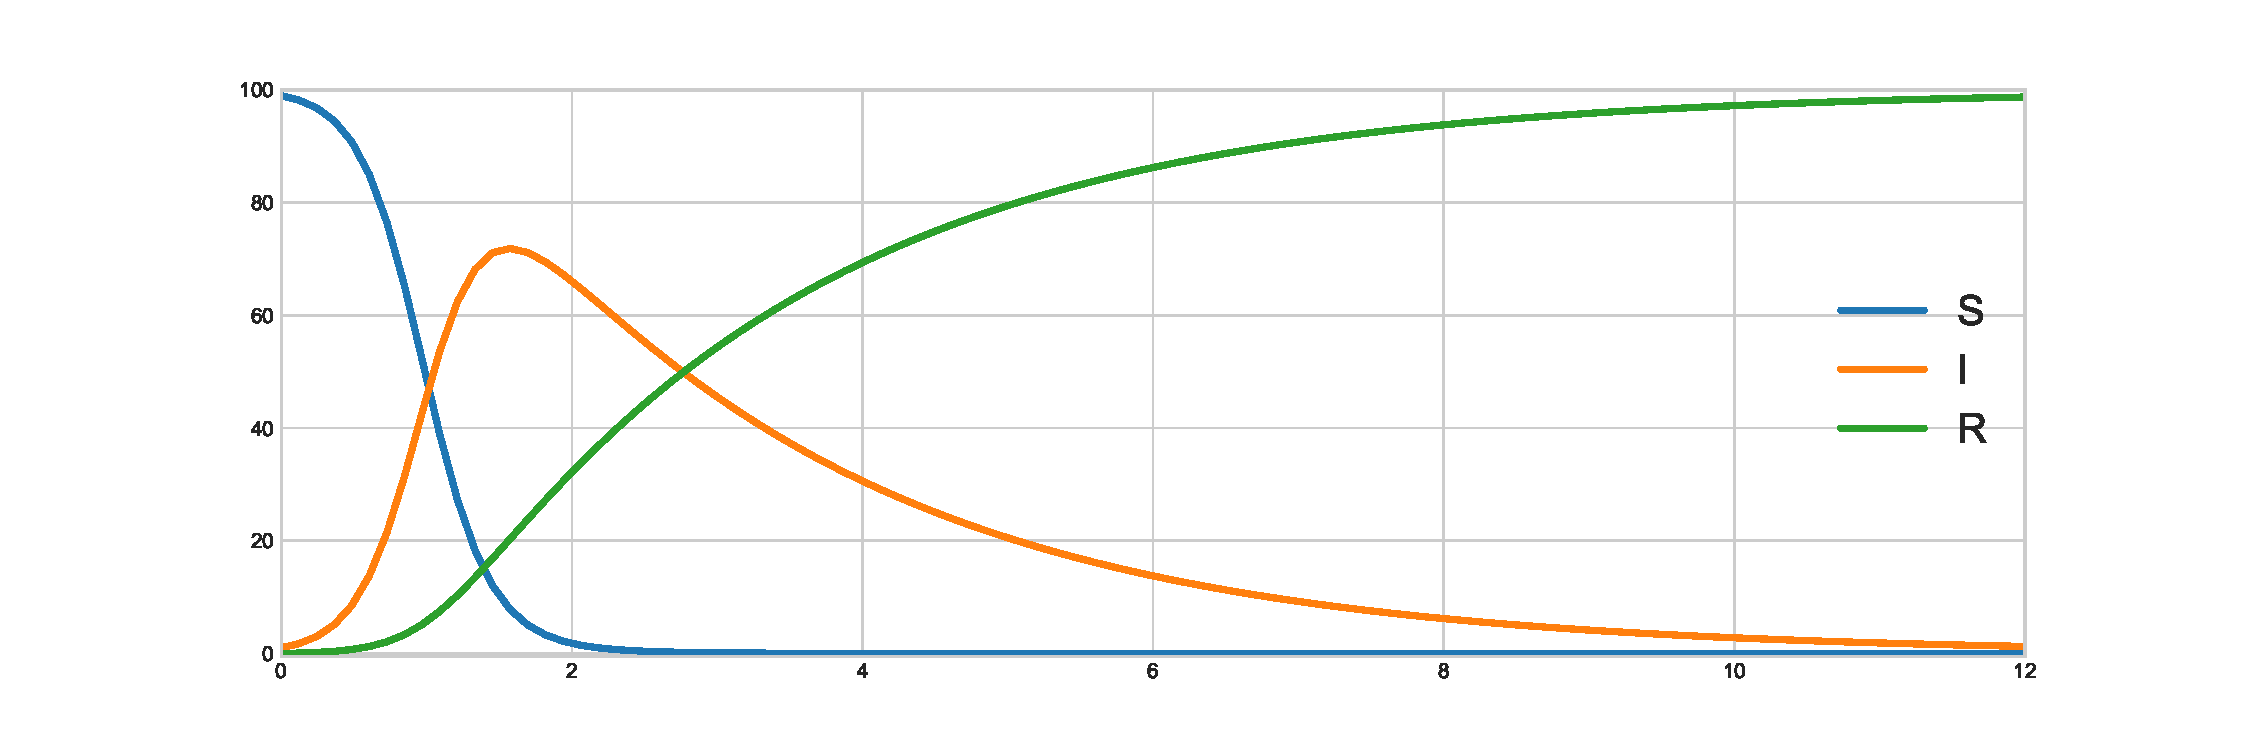
\includegraphics[width=0.7\textwidth]{SIR}
\end{center}
\end{frame}

\frame{
  \frametitle{Game Theory}
  \includestandalone[width=\textwidth]{hospitals}
}

\begin{frame}[fragile]

\begin{equation*}
\end{equation*}
  $$\bordermatrix{ & K_{2} = 0 & K_{2} = 40 & K_{2} = 65 & K_{2} = \infty \cr
  K_{1} = 0 & (59.6, 59.6) & (60.2, 59.6) & (51.8, 68.6) & (0.0, 119.0) \cr
  K_{1} = 40 & (59.6, 60.2) & (59.6, 59.6) & (50.6, 67.9) & (38.4, 80.9) \cr
  K_{1} = 65 & (68.6, 51.8) & (67.9, 50.6) & (59.6, 59.6) & (56.7, 62.5) \cr
  K_{1} = \infty & (119.0, 0.0) & (80.9, 38.4) & (62.5, 56.7) & (59.6, 59.6) \cr}$$
  \vspace{10mm}
  \pause
  \footnotesize{
  \begin{minted}{python}
    >>> import nash

    >>> g = nash.Game(-O1, -O2)
    >>> eqs = g.support_enumeration()
    >>> list(eqs)
    [(array([ 0.,  1.,  0.,  0.]), array([ 0.,  1.,  0.,  0.]))]
  \end{minted}
  }
\end{frame}

\begin{frame}
\frametitle{My PhD Work...}
\begin{center}
\includestandalone[width=0.7\textwidth]{ophcn_map}
\end{center}
\end{frame}

\begin{frame}[fragile]
\begin{minted}{bash}
pip install pandas
pip install numpy
pip install matplotlib
pip install scipy==0.19.1
pip install sklearn==0.17.1
pip install pulp==1.6.8
pip install networkx==1.11
pip install ciw==1.1.3
pip install nashpy==0.0.11
\end{minted}
\footnotesize{Emojis thanks to Twemoji.}
\end{frame}

\end{document}
